\documentclass[12pt,a4paper,oneside]{article}
\usepackage{geometry}
\geometry{a4paper,scale=0.7}
\usepackage{graphics}
\usepackage{indentfirst}
\usepackage{amsmath}
\usepackage{algorithm}
\usepackage{algorithmic}
\usepackage{bm}
\usepackage{setspace}
\usepackage{graphicx}
\usepackage{float}
\usepackage{CJKutf8}
\usepackage{hyperref}
\usepackage{color}
\usepackage{listings}

\definecolor{dkgreen}{rgb}{0,0.6,0}
\definecolor{gray}{rgb}{0.5,0.5,0.5}
\definecolor{mauve}{rgb}{0.58,0,0.82}

\author{Ruichen Wang}
\title{集成学习}
\begin{document}
\begin{CJK*}{UTF8}{gbsn}

\maketitle
\begin{abstract}
集成学习基础介绍
\end{abstract}

\tableofcontents

\section{Basic Concepts}
Ensemble的主要思想是训练多个模型,分别从不同的角度去解决同一个机器学习任务。一般来说,模型的误差主要来自三个方面:variance, bias 和noise。通过ensemble可以提高模型最终的稳定性,从而一定程度上减少这些误差。比较常见的ensemble方法有:
\begin{itemize}
\item Bagging
\item Boosting
\item Stacking
\item Blending
\end{itemize}


\section{Bias Variance Trade-off}

为什么要使用ensemble方法呢?直觉上,我们需要从多个角度来评估问题,多个模型能提供多个角度,所以能够更好的解决问题。

这里我们从数学上来证明多个模型的有效性。

假设我们要拟合的 $y_{target}$ 满足正态分布,$f$ 为理想模型, $\hat{f}$是训练得到的模型。$\epsilon$ 是一定的随机误差。那么有:
$$y=f(x)+\epsilon$$
$$\epsilon \sim N(0,\sigma^{2})$$
$$y \sim N(f(x), \sigma^{2})$$

假设我们用MSE来表示模型误差, 则可以写为:
\begin{align*}
Err(x) &=E \left[ \left(y-\hat{f}(x)\right)^{2} \right] \\ 
 &=E \left[y^{2} \right] + E \left[ \left(\hat{f}(x) \right)^{2} \right]-2E \left[y\hat{f}(x) \right]
\end{align*}

因为有$Var(x)=E\left[x^{2} \right] - E\left[x \right]^{2}$, 故有:

\begin{align*}
E\left[y^{2} \right] &= Var(y) + E\left[y \right]^{2} \\
&= \sigma^{2} +f^{2}
\end{align*}
$$E \left[ \left(\hat{f}(x) \right)^{2} \right] = Var\left( \hat{f}\right) + E\left[\hat{f} \right]^{2}$$
\begin{align*}
E \left[y\hat{f}(x) \right] &= E\left[(f+\epsilon) \hat{f} \right] \\
&= E\left[f \hat{f} \right] + E\left[\epsilon \hat{f} \right] \\ 
&= fE\left[ \hat{f} \right] +E\left[ \epsilon \right]E\left[ \hat{f} \right] \\
&= fE\left[ \hat{f} \right]
\end{align*}

合并可得:
\begin{align*}
Err(x) &= \sigma^{2} +f^{2} + Var\left( \hat{f}\right) + E\left[\hat{f} \right]^{2} -2 fE\left[ \hat{f} \right] \\
&= \left(f-E\left[\hat{f}\right] \right)^{2}+Var(\hat{f})+\sigma^{2} \\
&= Bias(\hat{f})^{2} +Var(\hat{f}) + \sigma^{2}
\end{align*}

对于任何模型,最终的目标就是最小化这个$Err(x)$。其中$\sigma^{2}$是无法避免的。它是数据本身存在的一定error。可以理解为bias 主要来源于没有足够好的hypotheses。 而variance主要来源于hypotheses太强。

我们希望有一个模型刚刚好可以拟合ground truth(完美的假设,最小化bias和variance)。但实际中,我们往往需要面对 bias variance trade-off。

\paragraph{*过拟合}: 模型表达能力强,bias低, variance高,模型更多的memorized the data。泛化能力差。

\section{Bagging Methods}
Bagging 是Boostrap Aggregating的缩写。也就是先 Boostrap 再 Aggregating。

抽样出多组数据,各自训练强分类器, 各自variance会很大, 然后采用bagging来降低variance。

\subsection{Boostrap Method (.632)}

有放回的均匀抽样,针对样本总体无法以正态分布来描述,常采用的方法。

假设给定的数据集包含d个样本。该数据集有放回地抽样$d$次,显然每个样本被选中的概率是$\frac{1}{d}$,因此未被选中的概率就是$\left( 1-\frac{1}{d}\right)$。这样一个样本在训练集中没出现的概率就是$d$次都未被选中的概率:$(1-\frac{1}{d})^{d}$。当$d$趋向无穷大时:
$$\mathop{lim} \limits_{d\to +\infty} (1-\frac{1}{d})^{d} = e^{-1} \approx 0.368$$
所以训练集中的数据大概就占原整体的63.2\%。所以也叫.632自助法

Aggregating 就是将上述方法重复i次,每次都得到一份数据,分别对每一份数据进行训练得到模型$f_{i}$, 最后所有模型投票来决定最终分类, 回归就是sum avg。

\subsection{Random Forest}
单棵树可以有很好的拟合能力。但是同样会产生较大的方差。Random Forest就是解决这个问题。

算法大概流程:
\begin{itemize}
\item .632采样生成一份bootstrap sample data。
\item 构造一棵决策树b,直到满足最大节点数(or 每个节点下只有k个sample):
\begin{itemize}
\item 从总特征p中随机选取一部分变量m (经验上, Classification:$\sqrt{p}$ , Regression: $\frac{p}{3}$)
\item 从m个变量中选择最佳变量/分叉点
\item 分割当前节点变为两个
\end{itemize}
\item 重复第二步N次
\end{itemize}

与bagging decision tree的区别:random forest每次随机选择特征。往往这样效果比 decision tree刻意选择的效果更好。有更好的泛化能力。

\subsection{Can Random Forest Overfitting? }
一个有意思的问题: 增加树的个数,最终bagging / random forest模型会不会过拟合?

这里我们简化问题到两个模型$f_{1}$,$f_{2}$进行bagging。bagging之后的模型为
$f=\frac{1}{2}f_{1}+\frac{1}{2}f_{2}$。
\begin{align*}
Var(f)&= Var(\frac{1}{2}f_{1}+\frac{1}{2}f_{2}) \\
&= \frac{1}{4}Var(f_{1})+\frac{1}{4}Var(f_{2})+2*\frac{1}{2}*\frac{1}{2}Cov(f_{1},f_{2})
\end{align*}

因为采用随机采样, $f_{1}$与$f_{2}$应为相互独立不相关,即$Cov(f_{1},f_{2})=0$。整体的方差减小到原来的一半。

也就是,random forest方法 "can not overfit data"。可以选择as many trees as you want。更合适的说法应该是,单棵树是可以过拟合的,增加树的个数并不会过拟合,只会让模型泛化误差更小(抗过拟合)。

\section{Boosting Methods}
Boosting是指能够将弱学习者转换为强学习者的集成算法。该类算法起源于针对一个理论的回答: 弱可学习问题和强可学习问题是否相等?

\subsection{Strongly Learnable vs. Weakly Learnable}
在概率近似正确(probably approximately correct,PAC)学习框架中:
\begin{itemize}
\item 如果算法正确率很高,强可学习。
\item 如果算法正确率仅比随机猜测略好,弱可学习。
\end{itemize}

Schapire后来证明了: 强可学习和弱可学习是等价的。 也就是说,在PAC学习的框架下,一个概念是强可学习的 充分必要条件 是这个概念是弱可学习的。

往往一个弱学习算法比强学习算法更容易实现。 而Boosting就是将多个弱学习分类器组合成一个强学习的方法。

boosting指的是sequential models, 将一系列弱模型(与bagging相反)串联起来组织一个强模型。所谓弱模型指的是模型略强于瞎猜。最后进行加权投票,weighted majority vote。注意boosting是有顺序的(seqentially)。所以不像bagging可以并行训练。

boosting希望每个弱模型尽量不相关。 那么我们理想条件下每个模型基于的训练数据都不相同。一种办法就是re-weight。

\subsection{AdaBoost}
AdaBoost的想法很简单, 希望$f_{1}$训练好后,$f_{2}$能很好的补充$f_{1}$的不足。换句话说, 也就是$f_{2}$ 希望让$f_{1}$表现的尽量差。

就像考试一样,总是希望别人不会的,自己会的那些题分值高。别人会的,自己不会的题最好不算分。那么我们应该如何修改题目的分值呢?

回想起弱学习器的定义,我们自然希望每次模型都尽量接近随机。对于正确的样本$p_{f=y}$,减少它的得分,对于错误的样本$p_{f\neq y }$,加大它的得分。所以我们定义的权重$w$应当满足:

$$\frac{\sum p_{f= y} / w}{\sum p_{f\neq y } * w+ \sum p_{f=y } / w} =0.5$$
定义错误率为$\epsilon= \frac{p_{f\neq y}}{p}$, 可得:
$$ \frac{1-\epsilon}{w} = \epsilon * w $$
$$w = \sqrt{\frac{1-\epsilon}{\epsilon}}$$

注意到我们的权重总是大于1的。(为什么?)

\paragraph{算法步骤}

\begin{itemize}
\item 初始化样本权重w = 1/N
\item 对于M个分类器分别: 
\begin{itemize}
\item 基于当前权重训练一个分类器$G_{m}(x)$
\item 计算错误率$\epsilon_{m}$
\item 计算 $\alpha_{m} = ln\left( \sqrt{\frac{1-\epsilon_{m}}{\epsilon_{m}}} \right)$
\item 更新错误分类的样本权重为$ p_{f\neq y }* e^{\alpha_{m}}$, 正确分类的样本权重为:$p_{f= y}* e^{- \alpha_{m}}$
\end{itemize}
\item 最终结果$G(x)=sign(\sum \alpha_{m} G_{m}(x))$。误分类少、表现优秀的模型权重大。
\end{itemize}

为什么要使用$\alpha$ 而不是$w$。 主要是为了计算起来更快一些,不再需要计算机做除法,表达起来也更方便。可以直接写成 $p_{t+1}=p_{t}*e^{-y*f*\alpha}$

\paragraph{缺点}

\begin{itemize}
\item 对于异常点很敏感,在噪声多的数据上表现不好
\item 算法结果不能表示概率 (指数loss)
\end{itemize}

\subsection{Bias and Variance of Boosting}
boosting是seqentially累加模型,自然就会导致模型之间强相关。套用上面bagging提到的公式,强相关的模型无法显著降低variance。更多的通过调整样本weight,降低bias来提升模型效果。


\subsection{Gradient Boosting}
GBDT其实就是Adaboost的一般数学推导,可以看成adaboosing一个泛化的方法。从梯数的思路去解决这个问题。

\paragraph{算法步骤}:
\newline

假设我们已经有一个累加分类器$G_{t-1}(x)$。希望找到一个新的$f_{t}$,$\alpha_{t}$, 来优化现有的的$G_{t-1}(x)$, $G_{t} = G_{t-1} + \alpha_{t}f_{t}$

最小化$Loss = \sum e^{-yG(x)}$,其中$G_{t} = G_{t-1} + \alpha_{t}f_{t}$。我们希望找到$\alpha$来最小化loss。
\begin{align*}
Loss &= \sum e^{\left(-y(g_{t-1}+\alpha*f)\right)} \\
&= \sum e^{-y*g_{t-1}}e^{-y*\alpha*f} \\
&= \sum_{y=f(x)} e^{-y*g_{t-1}}e^{\alpha} +  \sum_{y\neq f(x)} e^{-y*g_{t-1}}e^{-\alpha} \\ \\
\end{align*}
求导:$\frac{\partial L(g)}{\partial \alpha}=0$ , $\alpha= ln\sqrt{\frac{1-\epsilon}{\epsilon}}$
,和Adaboost完全一致。

说它是泛化的adabbost的原因就是这里的Loss是可以随便换的,l1/l2, exp, square loss 等等

\subsection{GBDT}
GBDT 就是boosting 模型使用decision tree。由于用的是残差,也就是累加,所以用于分类树是没有意义的。所以GBDT中的树都是回归树,不是分类树。

使用树作为子模型有很多好处,比如树可以处理missing feature,特征缺失对于树来说只是少了一些路径。对于outlier、噪音也不敏感。树的深度也方便调整等等

如果做的是regression, 常见的loss就是l2 loss。 如果是classification,常见的有KL、logloss等

\section{Blending}
将几个模型结果作为input feature。再加上一层LR。为了防止有的模型作弊(过拟合、欠拟合etc), 需要将训练数据再单独保存一份来训练LR。

\section{Stacking}
Stacking是个多层的多模型集合方法。每一层都可包括多个模型,下一层利用上一层模型的结果进行学习。

\begin{figure}[H]
\centering
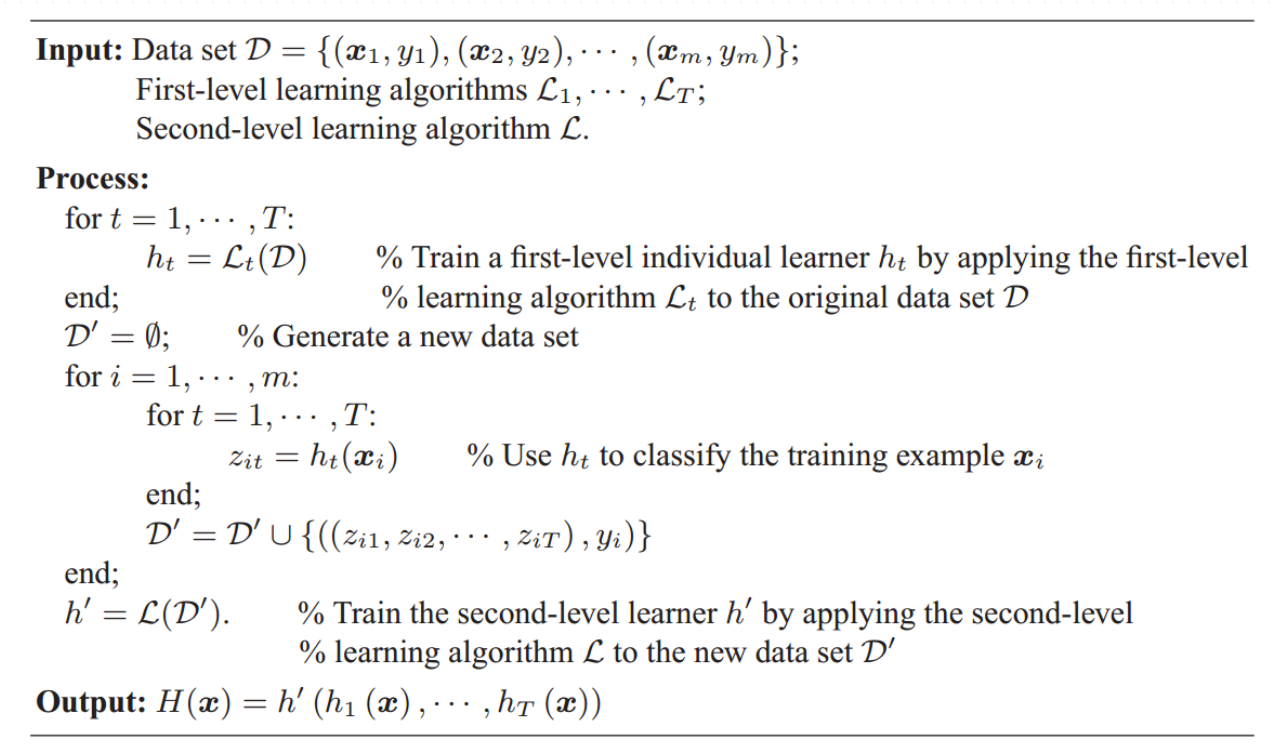
\includegraphics[width=6in,height=4in]{stacking}
\caption{Stacking 算法步骤}
\end{figure}



\end{CJK*}
\end{document}


























